\documentclass[12pt,titlepage]{article}
\usepackage{lmodern}
\usepackage[T1]{fontenc}
\usepackage[utf8]{inputenc}
\usepackage[francais]{babel}
\usepackage{amsfonts}
\usepackage{graphicx}
\usepackage{float}

\usepackage{geometry}
\geometry{hmargin=2.7cm,vmargin=2.5cm}
\newgeometry{left=3.8cm,right=2cm,top=2.5cm,bottom=2.5cm}

\graphicspath{{./}}

\title{Projet de Langages Web 2015 - M1 GIL}
\author{Thomas CAPET, Yohann HENRY}

\begin{document}
\maketitle
\newpage

\tableofcontents
\newpage

\section{Présentation du projet}

L'objectif du projet de Langages Web était de développer une plateforme web permettant de concevoir des quiz et d'y jouer.\\
Une notion d'utilisateur était demandée : l'administrateur a tous les droits, un utilisateur inscrit et connecté peut créer des quiz et y jouer, et un utilisateur anonyme peut jouer aux quiz déjà créés.\\
Enfin, pour plus de facilité dans le partage des quiz, il devait être possible de transmettre l'URL d'un quiz. Chaque quiz devait donc posséder son propre URL.
\medbreak
Notre site est adaptatif (\textit{responsive}) ; il s'adapte à la taille de l'écran, et fonctionne également sur portables.

\section{Mode d'emploi}

Le site possède une barre de menu horizontale, qui sera présente en haut de toutes les pages. Ce menu permet de retourner à l'accueil en cliquant sur \texttt{Quiz Constructor}, d'afficher la liste des quiz en cliquant sur \texttt{Quiz} et d'afficher la liste des utilisateurs inscrits en cliquant sur \texttt{Utilisateurs}. Egalement, si vous n'êtes pas connecté, il vous sera proposé à droite du menu de vous inscrire ou de vous connecter. Si vous êtes connecté, alors vous aurez la possibilité de vous déconnecter ou bien d'accéder à votre page de profil en cliquant sur votre identifiant.
\medbreak
Via la page d'accueil, vous pouvez \texttt{Commencer à jouer} et ainsi accéder à la liste de tous les quiz créés.
\medbreak
L'inscription se fait simplement. Après avoir cliqué sur \texttt{Inscription}, l'utilisateur arrive sur une page où il doit entrer un identifiant et un mot de passe.\\
Pour la connexion, il suffit de cliquer sur \texttt{Connexion}. L'utilisateur aura juste à rentrer son identifiant et son mot de passe, et la connexion s'effectuera.
\medbreak
Une fois la liste des quiz affichée, il vous est possible de jouer à n'importe lequel d'entre eux en cliquant sur son nom. S'affichera alors la liste de ses questions, à vous d'y répondre. Une fois toutes les questions répondues, le nombre de bonnes réponses vous sera transmis. Chaque quiz possédant une URL unique, un utilisateur peut le transmettre par mail ou par copier/coller.\\
Un utilisateur connecté aura également la possibilité, via la liste des quiz, d'éditer les quiz qu'il a créé. Un administrateur pourra modifier n'importe quel quiz.
\medbreak
La page d'édition des quiz et la page de création se ressemblent beaucoup. Il est possible de modifier la description du quiz, ainsi que les questions enregistrées pour ce quiz. Un utilisateur peut également rajouter des questions à un quiz qu'il a créé.\\
Pour créer un quiz, il suffira de se connecter et d'accéder à la liste des quiz. Un bouton \texttt{Créer un quiz} apparaîtra alors.
\medbreak
L'édition et la création des questions d'un sont similaires. L'utilisateur rentre ou modifie un intitulé (l'énoncé de la question), entre de 2 à 4 réponses pour cette question et indique quelle est la bonne réponse parmi les propositions entrées.
\medbreak
Via la liste des utilisateurs, il est possible d'accéder au profil de n'importe quel membre inscrit et, de son profil, aux quiz qu'il a créé.

\section{Fonctionnement global}

\begin{figure}[!h]
\centering
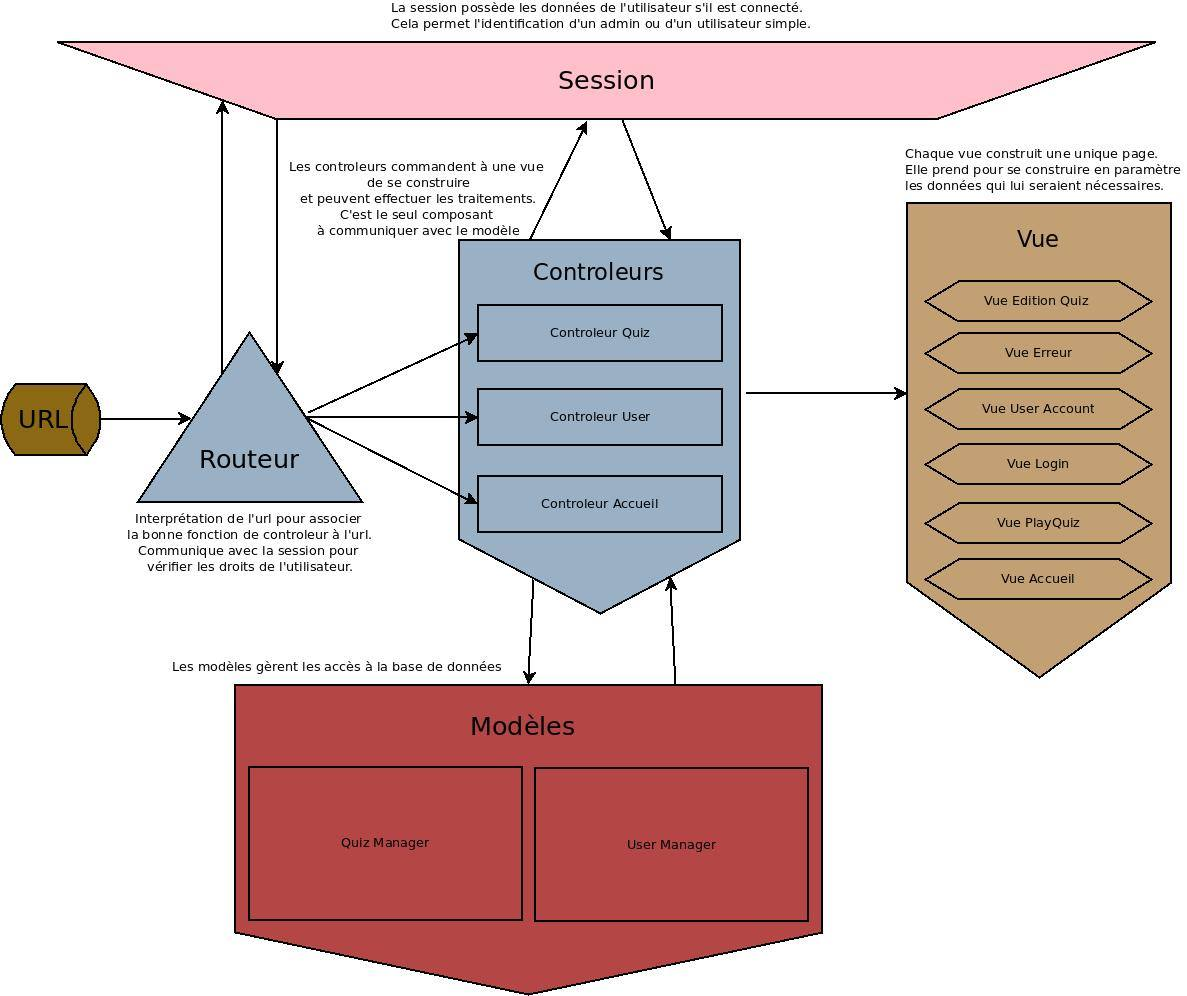
\includegraphics[width=16cm]{schemaFonctionnement.jpg}
\caption{Fonctionnement global}
\end{figure}

\newpage

\subsection{Routeur}

\subsection{Base de données}

\begin{figure}[!h]
\centering
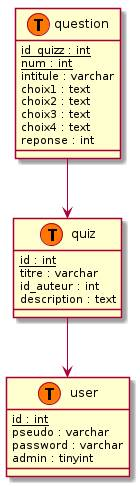
\includegraphics[height=15cm]{schemaBdd.jpg}
\caption{Base de données}
\end{figure}

\section{Technologie et langages utilisés}

\subsection{Langages utilisés}

Nous avons choisi de programmer en PHP, Javascript, HTML et CSS, car ces quatre langages sont des langages web que nous maitrisons bien.\\
Le PHP a l'avantage d'être orienté objet, ce qui nous a permis d'intégrer un patron MVC à notre projet.

\subsection{Bootstrap}

Bootstrap, ou Twitter Bootstrap, est un ensemble de code HTML et CSS permettant la mise en forme rapide des sites web.
\medbreak
Nous avons choisi de l'utiliser car il permet une grande rapidité de programmation en nous permettant de nous concentrer sur le fond plutôt que la forme. De plus, il permet de créer facilement un site web adaptatif (\texttt{responsive}), comme demandé dans les objectifs bonus du projet.
\medbreak
Il fonctionne en indiquant un ou plusieurs classes pour un élément. Il ira alors chercher dans son code CSS la mise en page nécessaire. L'imbrication de bloc \texttt{div} avec des classes est une fonctionnalité importe dans Bootstrap.

\end{document}

